\documentclass[10pt]{beamer}

\usetheme[progressbar=frametitle,numbering=none]{metropolis}
\usepackage{appendixnumberbeamer}

\usepackage{booktabs}

\usepackage{pgfplots}
\usepgfplotslibrary{dateplot}

\usepackage{xspace}
\newcommand{\themename}{\textbf{\textsc{metropolis}}\xspace}

\usepackage{graphicx}
\usepackage[absolute,overlay]{textpos}
\usepackage{cancel}
\usetikzlibrary{calc,positioning}

\title{EIP-4844: Proto-danksharding}
\subtitle{in-house protocol study, 4\textsc{pm} Roundtable}
\date{2024-06-05}
\author{Jeongho Jeon \& Youngbin Park}
\institute{DSRV (All That Node, WELLDONE Studio)}
\titlegraphic{\hfill\includegraphics[height=3.0ex]{dsrv_logo_master_black}}

\begin{document}

\maketitle

\begin{frame}[fragile]{Data Availability}
\begin{itemize}
  \item Availability -- can I use it when I want? \\
    for example, ``Open 10-9``, 99.99\%
  \item Can I read chain data when I want?
  \item Plasma L2 (commit-chains) post state hashes on L1
    periodically. \\
    If malicious L2 operators conceal L2 transaction
    details, public cannot prove L2 fraud. Plasma lacks
    data availability. \\
    see also Vitalik's talk at Ethereum Meetup (2017-09-20,
    \href{https://www.youtube.com/watch?v=OJT_fR7wexw}{YouTube})
  \item ``state'' means token balance, NFT ownership, and
    swap pool details, and so one.
  \item cf. Data Retrievability = Data Availability +
    historical archive
\end{itemize}
\end{frame}

\begin{frame}[fragile,t]{Rollup}
Rollup L2s write extra data (transactions or both changed
state and zero knowledge proofs) for public verification
in Ethereum L1.

Rollups are less scalable than Plasma due to extra data,
but offer data availability.

\begin{textblock*}{10cm}(2cm,4cm)
\includegraphics[trim={0 0 0 2.7cm},clip,scale=0.5]{rollup-centric-ethereum-roadmap.pdf}
\end{textblock*}
\end{frame}

\begin{frame}[fragile]{Expensive for L2s}
\includegraphics[trim={2.5cm 12cm 5.5cm 2cm},clip,scale=0.5]{ethereum-l2-data-fees.pdf}
\setlength{\TPHorizModule}{\textwidth}
\setlength{\TPVertModule}{\textwidth}
\begin{textblock}{0.2}(0.9,0.625)
{\tiny Dencun hardfork \\ on March 13, 2024 \par}
\end{textblock}
\begin{textblock}{0.2}(0.55,0.65)
{\scriptsize see also \href{https://l2fees.info/}{L2Fees.info}}
\end{textblock}
\end{frame}

\begin{frame}[fragile]{Blob}
\begin{itemize}
  \item 128 kbytes size
  \item up to 6 blobs in a block (maximum 2 Tb per year)
  \item separate gas system for blobs \\
    blob base fee goes up when more than 3 blobs in a block, \\
    blob base fee goes down when less than 3 blobs in a block.
  \item keep up to 4096 epochs (about 18 days, maximum 100 Gb) \\
    It is enough time to challenge and correct malicious L2. \\
    cf. EIP-4444 (History Expiry, chain data for 1 year only) is under discuss.
\end{itemize}
\end{frame}

\begin{frame}[fragile]{Ethereum storage types}
The lower the cheaper. (Below gas prices are simplified.)
\begin{footnotesize}
\begin{description}
  \item[STORAGE] (625 gas/byte $\times$ 10 gwei) ``state'' of smart contacts \\
    All nodes store STORAGE forever. \\
    Smart contracts can read and write STORAGE.
  \item[CALLDATA] (16 gas/byte $\times$ 10 gwei) input data for smart contacts \\
    L2s have used CALLDATA in the place of BLOB before dencun hardfork. \\
    Smart contracts can read CALLDATA. \\
    Vitalik proposed EIP-7706: Separate gas type for calldata last month.
  \item[LOG] (8 gas/byte $\times$ 10 gwei) events during smart contract execution \\
    Smart contacts write LOG, but cannot read.
  \item[TRANSIENT STORAGE] (3 gas/byte $\times$ 10 gwei, EIP-1153, new in dencun) \\
    Smart contracts can read and write TRANSIENT STORAGE, \\
    but discard it after transaction execution. \\
    cf. MEMORY (0.1 gas/byte $\times$ 10 gwei)
  \item[\colorbox{orange!20}{BLOB}] (1 gas/byte $\times$ 1 wei, EIP-4844, new in dencun) \\
    Nodes store BLOG for a while. \\
    Smart contacts cannot read and write BLOG.
\end{description}
\end{footnotesize}
\end{frame}

\begin{frame}[fragile]{Comparison to storage blockchains}
Storage blockchains focus on incentive, and prevent abusers
  that seek rewards while not providing storage. They use
  storage dedicated consensus like PoST (Proof of Spacetime).
  Complex computation may delay data retrieval. When the network
  has a few copies of data, it recovers copies.

EIP-4844 deals with smaller data than storage blockchains,
  and serves chain data without delay. It doesn't keep
  persistent data. \\ see also fisherman's dilemma.
\end{frame}

\begin{frame}[fragile]{In the future}
\begin{itemize}
  \item Users (i.e. L2s) and EL are not necessary of more major updates in
    \mbox{\cancel{Proto-}Danksharding}.
  \item will increase the number of blobs (32, 64, 128, 256 or 4096)
    while monitoring Ethereum network (EIP-7659 or EIP-7691) \\
    see also Youngbin's blob propagation latency chart
  \item may switch from KZG to something else (e.g. Merkle trees + STARK)
  \item DAS (Data Availability Sampling) -- all nodes do not need to store
    all blobs. nodes store a part of blobs, and a client can restore full blobs.
  \item Celestia, Avail, EigenLayer EigenDA, Starkware DAC
    (Data Availability Committee)/Validium/Volition, zkPorter, NEAR, \ldots
  \item Modular Blockchain -- consensus, execution, settlement,
    and data availability
\end{itemize}
\end{frame}

\begin{frame}[fragile]{LazyLedger and Celestia}
\begin{textblock*}{10cm}(1.2cm,0cm)
\includegraphics[trim={0 0 0 0},clip,scale=0.5]{fraud-and-data-availability-proofs.pdf}
\end{textblock*}
\end{frame}

\begin{frame}[fragile]{}
\begin{textblock*}{10cm}(1.2cm,1.5cm)
\includegraphics[trim={0 10cm 0 2.7cm},clip,scale=0.5]{bitcoin-cash-as-da-layer.pdf}
\end{textblock*}
\end{frame}

\section{Appendix}

\begin{frame}[fragile]{EIP-4844 blob transaction}
\scalebox{0.68}{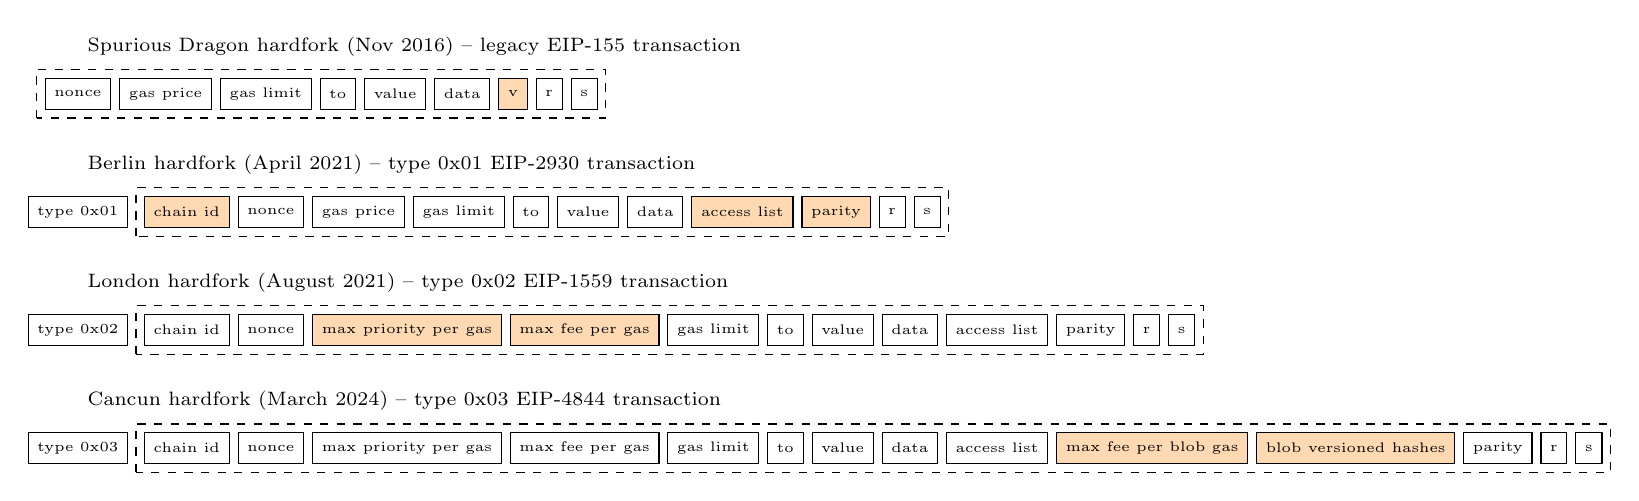
\begin{tikzpicture}
\tikzset{field/.style={shape=rectangle,draw,align=center,minimum height=0.4cm}}
\tikzset{array/.style={shape=rectangle,draw,minimum height=0.6cm}}
\def\sp{0.1cm}
\def\labely{0.6cm}
\def\ygap{1.5cm}
%
\node at (0cm,\ygap * 3 +\labely) [anchor=west,align=left] {\scriptsize Spurious Dragon hardfork (Nov 2016) -- legacy EIP-155 transaction};
\node at (0cm,\ygap * 3) [field] (nonce1) {\tiny nonce};
\node [field,right=\sp of nonce1] (gasprice1) {\tiny gas price};
\node [field,right=\sp of gasprice1] (gaslimit1) {\tiny gas limit};
\node [field,right=\sp of gaslimit1] (to1) {\tiny to};
\node [field,right=\sp of to1] (value1) {\tiny value};
\node [field,right=\sp of value1] (data1) {\tiny data};
\node [field,right=\sp of data1,fill=orange!30] (v1) {\tiny v};
\node [field,right=\sp of v1] (r1) {\tiny r};
\node [field,right=\sp of r1] (s1) {\tiny s};
\draw[dashed] ($(nonce1.south west)+(-\sp,-\sp)$) rectangle ($(s1.north east)+(\sp,\sp)$);
%
\node at (0cm,\ygap * 2 +\labely) [anchor=west,align=left] {\scriptsize Berlin hardfork (April 2021) -- type 0x01 EIP-2930 transaction};
\node at (0cm,\ygap * 2) [field] (type2) {\tiny type 0x01};
\node [field,right=\sp * 2 of type2,fill=orange!30] (chainid2) {\tiny chain id};
\node [field,right=\sp of chainid2] (nonce2) {\tiny nonce};
\node [field,right=\sp of nonce2] (gasprice2) {\tiny gas price};
\node [field,right=\sp of gasprice2] (gaslimit2) {\tiny gas limit};
\node [field,right=\sp of gaslimit2] (to2) {\tiny to};
\node [field,right=\sp of to2] (value2) {\tiny value};
\node [field,right=\sp of value2] (data2) {\tiny data};
\node [field,right=\sp of data2,fill=orange!30] (accesslist2) {\tiny access list};
\node [field,right=\sp of accesslist2,fill=orange!30] (parity2) {\tiny parity};
\node [field,right=\sp of parity2] (r2) {\tiny r};
\node [field,right=\sp of r2] (s2) {\tiny s};
\draw[dashed] ($(chainid2.south west)+(-\sp,-\sp)$) rectangle ($(s2.north east)+(\sp,\sp)$);
%
\node at (0cm,\ygap+\labely) [anchor=west,align=left] {\scriptsize London hardfork (August 2021) -- type 0x02 EIP-1559 transaction};
\node at (0cm,\ygap) [field] (type3) {\tiny type 0x02};
\node [field,right=\sp * 2 of type3] (chainid3) {\tiny chain id};
\node [field,right=\sp of chainid3] (nonce3) {\tiny nonce};
\node [field,right=\sp of nonce3,fill=orange!30] (maxprioritypergas3) {\tiny max priority per gas};
\node [field,right=\sp of maxprioritypergas3,fill=orange!30] (maxfeepergas3) {\tiny max fee per gas};
\node [field,right=\sp of maxfeepergas3] (gaslimit3) {\tiny gas limit};
\node [field,right=\sp of gaslimit3] (to3) {\tiny to};
\node [field,right=\sp of to3] (value3) {\tiny value};
\node [field,right=\sp of value3] (data3) {\tiny data};
\node [field,right=\sp of data3] (accesslist3) {\tiny access list};
\node [field,right=\sp of accesslist3] (parity3) {\tiny parity};
\node [field,right=\sp of parity3] (r3) {\tiny r};
\node [field,right=\sp of r3] (s3) {\tiny s};
\draw[dashed] ($(chainid3.south west)+(-\sp,-\sp)$) rectangle ($(s3.north east)+(\sp,\sp)$);
%
\node at (0cm,\labely) [anchor=west,align=left] {\scriptsize Cancun hardfork (March 2024) -- type 0x03 EIP-4844 transaction};
\node at (0cm,0cm) [field] (type4) {\tiny type 0x03};
\node [field,right=\sp * 2 of type4] (chainid4) {\tiny chain id};
\node [field,right=\sp of chainid4] (nonce4) {\tiny nonce};
\node [field,right=\sp of nonce4] (maxprioritypergas4) {\tiny max priority per gas};
\node [field,right=\sp of maxprioritypergas4] (maxfeepergas4) {\tiny max fee per gas};
\node [field,right=\sp of maxfeepergas4] (gaslimit4) {\tiny gas limit};
\node [field,right=\sp of gaslimit4] (to4) {\tiny to};
\node [field,right=\sp of to4] (value4) {\tiny value};
\node [field,right=\sp of value4] (data4) {\tiny data};
\node [field,right=\sp of data4] (accesslist4) {\tiny access list};
\node [field,right=\sp of accesslist4,fill=orange!30] (maxfeeperblobgas4) {\tiny max fee per blob gas};
\node [field,right=\sp of maxfeeperblobgas4,fill=orange!30] (blobversionedhashes4) {\tiny blob versioned hashes};
\node [field,right=\sp of blobversionedhashes4] (parity4) {\tiny parity};
\node [field,right=\sp of parity4] (r4) {\tiny r};
\node [field,right=\sp of r4] (s4) {\tiny s};
\draw[dashed] ($(chainid4.south west)+(-\sp,-\sp)$) rectangle ($(s4.north east)+(\sp,\sp)$);
\end{tikzpicture}}
\end{frame}

\begin{frame}[fragile]{New block fields}
\texttt{blob\_gas\_used} and \texttt{excess\_blob\_gas} are new in EL block (execution payload).

\texttt{blob\_kzg\_commitments} is new in CL block (beacon block).

There are no blobs in transactions and blocks.
Both contain blob references only.
There are blob hashes in a transaction.
There are blob commitments in a beacon block.
\end{frame}

\begin{frame}[fragile]{New precompile and opcodes}
New precompile \texttt{point\_evaluation\_precompile} takes
  versioned hash + x + y + KZG commitment + KZG proof, and
  checks 1) whether a versioned hash corresponds to a committed
  polynomial and 2) whether a proof proves that $f(x) = y$.

It is useful for ZK-rollups. It can check whether a correct
  blob was used as a input of ZKP system efficiently.
  By the way, precompiles for BLS12-381 (EIP-2537) are planed in
  next hardfork, Pectra.

New opcode \texttt{BLOBHASH} pops a blob index, and pushes
  a blob versioned hash on the stack.

The \texttt{BLOBBASEFEE} opcode of EIP-7516 (in dencun hardfork)
allows smart contracts access blob base fee of the current block.
\end{frame}

\begin{frame}[fragile]{KZG commitment and proof 1/2}
A blob consists of 4096 field elements (each 32 bytes).
We convert a blob into a polynomial by Lagrange interpolation:
$f(0) = \text{first element},\,f(1) = \text{second element}, \ldots,\,f(4095) = \text{last element}$.

Over 141k people participated in KZG ceremony last year, and
generated $g_1^s$, $g_1^{s^2}$, \ldots, $g_1^{s^{4095}}$, and
$g_2^s$, $g_2^{s^2}$, \ldots, $g_2^{s^{64}}$. Joonkyo and Hyunggi contributed
\href{https://github.com/dsrvlabs/czg-keremony}{czg-keremony} at that time.
We can compute $g_1^{f(s)}$, and it is the KZG commitment of a blob.
You can regard KZG commitment as a blob's hash.

If you want to prove $f(x) = y$, calculate a KZG proof $\pi$.
Anyone can verify that $f(x) = y$ efficiently with KZG commitment and proof
without evaluating a polynomial costly.
And KZG proofs are aggregatable and ZKP-friendly, too.

$x$ is a random point ideally. In practice, we use the hash of
prefix + blob + KZG commitment as $x$.
\end{frame}

\begin{frame}[fragile]{KZG commitment and proof 2/2}
KZG proof $\pi = g_1^\frac{f(s) - y}{s - x}$

verify a ZKG proof: $e(\pi, g_2^s / g_2^x) = e(\text{commitment} / g_1^y, g_2)$

\begin{align*} 
e(\pi, g_2^s / g_2^x) &= e(g_1^\frac{f(s) - y}{s - x}, g_2^s / g_2^x) \\
 &= e(g_1,  g_2^{s - x})^\frac{f(s) - y}{s - x} \\
 &= e(g_1, g_2)^{\frac{f(s) - y}{s - x} \cdot (s - x)} \\
 &= e(g_1, g_2)^{f(s) - y} \\
e(\text{commitment} / g_1^y, g_2) &= e(g_1^{f(s)} / g_1^y, g_2) \\
 &= e(g_1^{f(s) - y}, g_2) \\
 &= e(g_1, g_2)^{f(s) - y}
\end{align*}

pairing: $e(a^2, b) = e(a\cdot a, b) = e(a, b)\cdot e(a, b) = e(a, b)^2 = e(a, b^2)$
\end{frame}

\begin{frame}[fragile]{Blob terms 1/3}
\begin{description}
  \item[blob] (128 kb) blob itself
  \item[KZG commitment] (48 bytes) convert blob to polynomial,
    and evaluate at trusted setup point \\ CL's blob reference
  \item[KZG proof] (48 bytes) convert blob to polynomial,
    and evaluate at the point that is determined by
    blob and KZG commitment
  \item[versioned hash] (EVM-friendly 32 bytes) \\
    {[version prefix (0x01) + hash of KZG commitment]} \\
    EL's blob reference
\end{description}
\end{frame}

\begin{frame}[fragile]{Blob terms 2/3}
\begin{description}
  \item[network form] [RLP-encoded array of blob transaction + blobs +
    KZG commitments + KZG proofs] \\ EL's representation
  \item[blob bundle] [JSON object of KZG commitment + KZG proof + blob] \\
    from EL to block proposer CL
  \item[blob sidecar] [SSZ-encoded container of beacon block root +
    blob index in block + blob + KZG commitment + KZG proof +
    signed beacon block header + KZG commitment inclusion proof] \\
    CL's representation
\end{description}
\begin{textblock*}{10cm}(0cm,6.75cm)
\includegraphics[trim={0 0 0 0},clip,scale=0.18]{sylvanian-families-sidecar.jpg}
\end{textblock*}
\end{frame}

\begin{frame}[fragile]{Blob terms 3/3}
\begin{description}
  \item[KZG commitment inclusion proof] used in the blob sidecar \\
    {[Merkle proof of blob KZG commitments field in a beacon block
    on the top of Merkle proof of this KZG commitment among KZG commitments]} \\
    proves that this KZG commitment is contained in this beacon block. \\
    useful for light clients. \\
    this proof lacks left-rightness because blob index tells on which side
    the node is. \\
    blob KZG commitments field has the SSZ list type, and SSZ
    Merkleization mix\_in\_length hashes the list Merkle root with its length
    (i.e. the number of blobs in a block).
\end{description}
\end{frame}

\begin{frame}[fragile]{Step-by-step (Thanks, Youngbin :)}
\begin{description}
  \item[user (L2 sequencer)] calls \texttt{eth\_sendRawTransaction}
    JSON-RPC method, uses \emph{network form}
  \item[RPC server] $\Downarrow$ \\
    p2p transfer by \texttt{NewPooledTransactionHashes}
    messages, additional info (tx type and size) in
    eth/68 \texttt{NewPooledTransactionHashes} message,
    uses \emph{network form}
  \item[EL clients] $\Downarrow$ \\
    puts \emph{blob bundles} in
    \texttt{engine\_getPayloadV3} response
  \item[proposer CL] $\Downarrow$ \\
    broadcasts \emph{blob sidecars} via
    gossipsub p2p, or requests blob sidecars explicitly by
    \texttt{BlobSidecarsByRoot} and \texttt{BlobSidecarsByRange}
  \item[CL clients] check whether blob is available by
    \texttt{is\_data\_available(beacon\_block\_root, blob\_kzg\_commitments)}
\end{description}
\end{frame}

\begin{frame}[b,fragile]{DAS}
2D Reed-Solomon encoding

Reed-Solomon (RS) codes

TCP/IP network corrects data corruption. \\
Why use it? To prevent tampering

Attackers should withhold more than 1/4 data to make data unavailable.
It can be detected by a small number of probes.

see also PeerDAS, SubnetDAS, LossyDAS, IncrementalDAS, DiDAS, FullDAS designs.
\begin{textblock*}{10cm}(7.5cm,1cm)
\includegraphics[page=13,trim={7cm 5.8cm 7cm 14cm},clip,scale=0.70]{fraud-and-data-availability-proofs.pdf}
\end{textblock*}
\end{frame}

\end{document}
